\documentclass[11pt]{article}

\usepackage[margin=1.1in]{geometry}
\usepackage{amsmath}
\usepackage{amssymb}
\usepackage{amsthm}
\usepackage{booktabs}
\usepackage{graphicx}
\usepackage{microtype}
\usepackage[round,authoryear]{natbib}
\usepackage[colorlinks=true,allcolors=blue]{hyperref}

\newtheorem{proposition}{Proposition}

\title{\textbf{Win Nodes for Bayes Nets:\\ Exact Order-Statistic
Queries on Gaussian Graphical Models}}
\author{Peter Cotton}
\date{\normalsize First version: September 6, 2026. This version: November 7, 2026.}

\begin{document}
\maketitle

\begin{abstract}
\noindent The inference stack of a Gaussian graphical model returns
marginals, joint moments and samples, and none of these answers the
questions a user of a correlated field most often asks: which
component is the maximum, when is a threshold first crossed, who
wins. We formalize these as the queries of a \emph{win node}, an
$n$-ary node $W=\arg\min_i X_i$ adjoined to Gaussian variables. On
chains and banded precisions, where the graphical-model libraries
stop at marginals, the classical recursions give the maximum and
first passage in linear work, and we add exact marginals of the time
of the maximum.
A rating model supplies the demonstration: latent ability paths with
match results as evidence give a Laplace posterior that is a
Gauss--Markov chain, and the peak-career query on 129{,}559 ATP
matches returns a bimodal law for Nadal and a non-interval credible
set for Agassi, neither of which any summary of the marginals
contains.
\end{abstract}

\section{Queries that are not marginal functionals}

Let $X=(X_1,\dots,X_n)$ be jointly Gaussian: the setting of the
Kalman filter, the Gaussian Markov random field, and the Gaussian
belief-propagation stack. Every mainstream toolkit returns marginal
moments, covariances, samples, and evidence. Four common queries are
functionals of the joint law that no collection of low-dimensional
marginals determines.

\begin{enumerate}
\item Argmax marginals $a_t=\Pr(X_t=\max_s X_s)$: which sensor reads
the extreme, which index carries the peak, which entrant wins.
\item The law of the maximum $F_M(u)=\Pr(\max_t X_t\le u)$, whose
complement is the excursion probability of spatial statistics.
\item First passage, the distribution of $\tau=\min\{t:X_t>u\}$:
sequential monitoring, degradation to failure, barrier crossing.
\item Top-$k$ membership $\Pr(X_i \text{ among the } k \text{
smallest})$: shortlists, portfolio inclusion, admission.
\end{enumerate}

The stationary AR(1) chain makes the gap concrete. Take
$X_{t+1}=\phi X_t+\sqrt{1-\phi^2}\,\epsilon_t$ with $X_1\sim N(0,1)$:
every marginal is $N(0,1)$, and a stationary Kalman filter reports
exactly that at every index. The argmax marginals at $\phi=0.9$,
$n=20$, computed by the method of Section~\ref{sec:chain} and
verified against $4\times10^5$-path Monte Carlo to $0.007$, put mass
$0.091$ on each endpoint and $0.035$ in the middle. Interior points
are squeezed by correlated-high neighbours on both sides; endpoints
have one neighbour. The fact lives in the joint law, so the marginal
layer cannot state it.

We call the object that answers these queries a \emph{win node}: a
deterministic $n$-ary node $W=\arg\min_i X_i$ (min-wins; negate for
utilities) adjoined to the Gaussian variables, together with its
order-statistic relatives. The definition is trivial. The
observation of this paper is that for the two coupling structures
that dominate practice, the node's forward query, its derivatives,
and its conditioning rule are exact and cheap at the same time,
which is what a graphical-model query type requires.

The ingredients are classical, and we say so once. The
one-dimensional winning-time integral is the random-utility
representation of \citet[eq.~4.7]{domencich1975}; the shared survival field
is competing-risks calculus; the transfer operator on a Markov chain
is the sum-product algorithm; the derivative identity of
Section~\ref{sec:factor} was reached for absolutely continuous
joint laws by \citet{muller2022}. The lattice engine that evaluates and inverts
these objects at scale, with its covariance grammar and tie-density
Jacobians, is \citet{cotton2026}, on which this paper builds
throughout. Recursive grid integration, which gives orthant, maximum
and first-passage probabilities when a density factors over adjacent
variables, goes back to sequential analysis \citep{armitage1969}.
\citet{hayter2006} develops it for Markov and higher-order
dependence, \citet{miwa2003} build general orthant probabilities from
it, and \citet{basak2004} obtain level crossings of AR($p$) processes
through their state-space representations. What is new here is the argmax layer on a chain:
exact marginals of the time of the maximum for an inhomogeneous,
data-conditioned Gauss--Markov chain, a discrete counterpart of the
path decomposition at the maximum of \citet{mori2021}; and the
demonstration that a whole-history rating posterior \citep{coulom2008}
is one of its inputs, which gives the posterior law of a career peak
without sampling.

\section{Adjacent machinery}

TrueSkill \citep{herbrich2007} is a Bayes net with win nodes
already: its factor graph attaches greater-than factors to
performance differences and propagates moment-matched messages. Its
win node is binary, multi-entrant events are chains of comparisons
between adjacent ranks, and the factor itself is approximated by expectation
propagation. Section~\ref{sec:observed} gives the exact $n$-ary
likelihood message; the TrueSkill factor is its $n=2$ case.

Modern Gaussian message-passing systems and GMRF libraries compute
marginals, free energies and samples for very large models. Their
query vocabularies do not include the four functionals above. The
win node is proposed as an addition to that vocabulary, not as a
competitor to the toolkits.

For latent Gaussian models, \citet{bolin2015} compute excursion sets
and exceedance probabilities by sequential importance sampling,
implemented in the R package \texttt{excursions}
\citep{bolin2018}. On chains
and bands the same functionals admit the deterministic pass of
Section~\ref{sec:chain}. Simulation remains the recourse for general
sparsity, and our software points there at its refusal boundary.

GHK evaluates one orthant probability per alternative by sequential
importance sampling. \citet{ridgway2016} showed that on an AR(1)
covariance its normalized variance grows exponentially in dimension.
That is the chain case, where the restricted transfer operator is
exact and linear in $n$; Section~\ref{sec:checks} measures its
accuracy, which is tightest at high correlation.

\section{The win node on factor-structured fields}
\label{sec:factor}

The factor case is settled and we use it rather than develop it.
The shared-field construction and its lattice discipline are
\citet[\S3]{cotton2026}. Let
$X=\mu+Vf+\mathrm{diag}(\sqrt{D})\,\epsilon$ with $f\sim N(0,I_r)$.
Conditional on $f$ the components are independent, so
\begin{equation}
a_i \;=\; \Pr(X_i=\min_j X_j)
\;=\; \mathbb{E}_f\!\int f_i(x)\prod_{j\ne i}S_j(x)\,dx ,
\label{eq:win}
\end{equation}
with $S_j$ the conditional survival of $X_j$. In English: component
$i$ wins by finishing at some value $x$ with everyone else still
above it, averaged over the shared luck. The product is shared, so
building $L(x)=\sum_j\log S_j(x)$ once on a lattice of $L$ points
prices every component by the subtraction $e^{L-\log S_i}$, at
$O(nLQ)$ for a $Q$-node quadrature.

\citet[\S5]{cotton2026} shows the derivative to be the tie density
on the face where $i$ and $j$ tie, so the Jacobian is minus a
weighted graph Laplacian and applies in $O(nL)$ without forming an
edge; \citet{muller2022} reach the same identity for absolutely
continuous joint laws through the surplus function. \citet{cotton2026b} develops this case as the posterior
probability of optimality for factor-Gaussian beliefs, including the
comparison against marginal-only surrogates and the bandit and
stopping consequences. We take it as given here and spend the paper
on the structure it does not cover.

\section{Conditioning on who won}
\label{sec:observed}

A query node becomes a Bayes-net citizen when it can be observed.
Condition on $W=k$ and integrate out the factor and the winner's own
noise $z$:
\begin{equation}
\Pr(W=k\mid\mu)\;=\;\mathbb{E}_{f,z}\prod_{j\ne k}
\Phi\!\left(\frac{\mu_k-\mu_j+(Vf)_k-(Vf)_j+z\sqrt{D_k}}
{\sqrt{D_j}}\right).
\label{eq:obslik}
\end{equation}
In English: given the shared luck and the winner's own performance,
each rival independently had to finish behind, and each such event
is one normal CDF.

The score of \eqref{eq:obslik} is analytic: posterior node weights
times Mills ratios, one extra pass over arrays the likelihood
already computes. The message an observed win node passes to its
Gaussian parents therefore carries exact first-order information. At
$n=2$ and $r=0$ the likelihood reduces to
$\Phi\!\left((\mu_k-\mu_j)/\sqrt{D_k+D_j}\right)$, the win
probability under TrueSkill's greater-than factor with zero draw
margin. The $n$-ary node needs no pairwise
chaining and no moment approximation of the factor itself; moment
approximations enter only if the user chooses a Gaussian posterior
family, exactly as in expectation propagation. The likelihood is the multinomial
probit likelihood, and it with its analytic score is the estimation
core of \citet[\S5]{cotton2026}; we use it to generate a posterior
rather than as a contribution. The implementation here agrees with
finite differences and with dual-number automatic differentiation at
$10^{-10}$.

\section{The order-statistic layer on chains and bands}
\label{sec:chain}

Now let the coupling be Markov with precision bandwidth $b$; the
Gauss--Markov chain is $b=1$. Write the chain as $X_1\sim
N(\mu_1,\sigma_0^2)$ and $X_{t+1}\mid X_t\sim
N(\mu_{t+1}+\phi_t(X_t-\mu_t),s_t^2)$. A tridiagonal precision
matrix delivers these parameters directly: its Cholesky factor is
bidiagonal, and each row is a conditional regression.

\emph{Max-CDF and first passage.} The lattice conventions are those
of \citet[\S3]{cotton2026}, and the pass is the recursive
integration of \citet{hayter2006} on that lattice. Restrict the
transfer operator below $u$. With $T_t$ the transition kernel on the lattice and
$\pi_u$ the initial sub-density cut at $u$,
\begin{equation}
\Pr(\max_{s\le t}X_s\le u)\;=\;\mathbf{1}^\top
\Big(\prod_{s<t}T_s^{(u)}\Big)\pi_u,
\qquad T^{(u)}(x'\mid x)=T(x'\mid x)\,\mathbf 1\{x'\le u\},
\end{equation}
one forward pass, $O(nL)$ per threshold with banded kernels. The
survivor-mass decrements of the same pass are the first-passage law.
Integrating the survival of the max over a threshold grid gives
$\mathbb E[\max]$; the rectangle rule biases this by $O(\Delta u)$,
measured at $+0.053$ on a ten-node chain, and the trapezoid removes
it. A hard cell cutoff at $u$ costs $O(\Delta x)$; assigning the
boundary cell its fractional occupancy restores $O(\Delta x^2)$,
which is the difference between $10^{-2}$ and $2\times10^{-4}$
agreement with the i.i.d.\ closed form at 400 lattice points.

\emph{Argmax marginals.} For each lattice threshold $u_k$, a forward
pass restricted strictly below $u_k$ and reaching $X_t=u_k$ gives
$\alpha_t(k)=\Pr(X_1,\dots,X_{t-1}<u_k,\ X_t=u_k)$, and a backward
conditional pass gives $\beta_t(k)=\Pr(X_{t+1},\dots,X_n<u_k\mid
X_t=u_k)$. Then
\begin{equation}
\Pr(X_t=\max_s X_s)\;=\;\sum_k \alpha_t(k)\,\beta_t(k),
\end{equation}
integrating out the value of the maximum. With transitions
precomputed the double pass is matrix slices, $O(nL^2)$ in total.

\emph{Bandwidth $b$ by state lifting.} The vector
$(X_t,\dots,X_{t+b-1})$ is Markov, so the same restricted passes run
on the lifted state at $O(nL^{b+1})$: linear in $n$, exponential
only in the bandwidth. At $b=2$ the lift covers AR(2), including the
cyclical regime with complex roots that has no $b=1$ analogue. With
the second coefficient set to zero the lift reproduces the $b=1$
pass to $5.6\times10^{-16}$ on the same grid.

\section{Numerical checks}
\label{sec:checks}

All numbers come from committed, seeded scripts in the public
repository. Monte Carlo appears only as a referee.

\begin{center}
\begin{tabular}{llll}
\toprule
query & setting & exact vs.\ referee & cost \\
\midrule
max-CDF & AR(1), $n{=}50$, $\phi{=}0.99$ & $5\times10^{-3}$ (MC $4{\times}10^5$) & 3 ms \\
max-CDF & i.i.d.\ closed form, $n{=}12$ & $2\times10^{-4}$ & --- \\
argmax & AR(1), $\phi{=}0.9$, $n{=}20$ & $7\times10^{-3}$ (MC) & ms \\
argmax & random walk, $n{=}40$ & $4\times10^{-3}$ (MC) & ms \\
band $b{=}2$ & AR(2) incl.\ cyclical & $1.1\times10^{-2}$ (grid-limited) & 230 ms/thr. \\
$b{=}2$ embed & $\phi_2{=}0$ vs.\ $b{=}1$ & $5.6\times10^{-16}$ & --- \\
first passage & inhomogeneous chain, $n{=}10$ & $5\times10^{-3}$ (MC) & $O(nL)$ \\
$\mathbb E[\max]$ & same & $5\times10^{-3}$ (MC band) & --- \\
\bottomrule
\end{tabular}
\end{center}

\emph{Tail thresholds.} At a low threshold the max-CDF is an orthant
probability, $\Pr(X_1\le u,\dots,X_n\le u)$, and as $u$ falls it
becomes a rare event. A direct sampler needs about $1/p$ draws to see
it at all, and on this AR(1) structure the variance of GHK, which
computes such orthants, grows exponentially in $n$
\citep{ridgway2016}. The restricted pass costs the
same whatever $p$ is: 66 ms per threshold here.

\begin{center}
\begin{tabular}{lllll}
\toprule
$u$ & exact, $L{=}400$ & exact, $L{=}800$ & $10^6$ draws & draws for
10\% error \\
\midrule
$0.0$  & $6.471\times10^{-3}$ & $6.465\times10^{-3}$ & $6.432\times10^{-3}$ & $1.5\times10^{4}$ \\
$-1.0$ & $1.753\times10^{-5}$ & $1.752\times10^{-5}$ & $1.60\times10^{-5}$ (16 hits) & $5.7\times10^{6}$ \\
$-1.5$ & $3.067\times10^{-7}$ & $3.079\times10^{-7}$ & no hits & $3.2\times10^{8}$ \\
$-2.0$ & $2.520\times10^{-9}$ & $2.521\times10^{-9}$ & no hits & $4.0\times10^{10}$ \\
$-2.5$ & $9.380\times10^{-12}$ & $9.418\times10^{-12}$ & no hits & $1.1\times10^{13}$ \\
$-3.0$ & $1.576\times10^{-14}$ & $1.578\times10^{-14}$ & no hits & $6.3\times10^{15}$ \\
\bottomrule
\end{tabular}
\end{center}

Stationary AR(1), $n=50$, $\phi=0.9$. Simulation agrees where it has
hits and returns zero where it does not, which is an absence of
information rather than a small error. Below $u=-1.5$ no referee is
available at all, and the evidence for the exact values is that they
are stable under grid refinement: the two passes agree to three or
four significant figures at every threshold, including
$1.58\times10^{-14}$.

Two consequences follow from the argmax table rather than merely
illustrating it. The boundary pile-up law is one: positive serial
correlation pushes the argmax of a stationary path to the endpoints,
$2.6\times$ at $\phi=0.9$, and no marginal summary can express this.
The finite-$n$ arcsine refinement is the other. On a random walk the
transfer operator matches the finite-$n$ argmax law to $0.3\%$ while
the continuum arcsine density sits $1\%$ away, because the engine
computes the exact finite law of which arcsine is the limit. The
same pass handles the drifted, barriered and mean-reverting cases
that have no closed form. The accuracy profile is complementary to
simulation: the exact pass is tightest at high correlation, and its
cost is linear in $n$ where the GHK variance on an AR(1) grows
exponentially \citep{ridgway2016}.

\section{Peak seasons from win evidence}
\label{sec:tennis}

A rating model is a Bayes net whose evidence is wins, and it produces
exactly the posterior this paper queries. The model is the
whole-history rating of \citet{coulom2008}, with a probit link in
place of its logistic one: one player has a latent
ability path $\theta_1,\dots,\theta_T$ across the years of a career
under a random-walk prior. Each match against an opponent of
ability $a_o$ contributes $\log\Phi(\pm(\theta_t-a_o))$ by
\eqref{eq:obslik} at $n=2$, a term touching one year, so the
likelihood's Hessian is diagonal. The prior's precision is
tridiagonal, as \citet{coulom2008} observed for each player's path,
the Laplace posterior
precision is their sum, and the
career posterior is therefore a Gauss--Markov chain of the kind
Section~\ref{sec:chain} reads.

The data are 129{,}559 ATP matches from 1985 to 2024 and the 1{,}453
players with at least fifteen of them. Static abilities for the field
come from a MAP fit of the probit Bradley--Terry likelihood. One
player at a time then has that constant replaced by a yearly path,
fitted under the random-walk prior with the innovation scale chosen
by the Laplace marginal likelihood. Opponents stay at their static
strength, which is a conditioning step rather than a joint fit.

Reading the peak off the fitted path is what a rating table invites.
The argmax marginals answer the question that was asked.

\begin{center}
\begin{tabular}{lccl}
\toprule
player & fitted peak & $\Pr(\text{that year})$ & 80\% credible set \\
\midrule
Federer  & 2006 & 0.52 & 2005--2006 \\
Nadal    & 2013 & 0.27 & six years within 2008--2019 \\
Djokovic & 2015 & 0.43 & 2013--2015 \\
Sampras  & 1994 & 0.47 & 1994--1996 \\
Agassi   & 1995 & 0.55 & 1995, 2002--2003 \\
Murray   & 2016 & 0.59 & three years within 2009--2016 \\
\bottomrule
\end{tabular}
\end{center}

The point answers are the ones a reader would expect, and stating
them alone would overclaim. Federer's 2006 carries $0.52$ against
$0.41$ for 2005. Nadal's most likely peak year carries $0.27$, and
his law is bimodal: $0.267$ at 2013 and $0.220$ at 2018, with the
years between them small. Agassi's credible set is not an interval.
It holds 1995 and the 2002--2003 resurgence and excludes the years
in between, which is a statement about the joint law and not about
any year's marginal.

\begin{figure}[t]
\centering
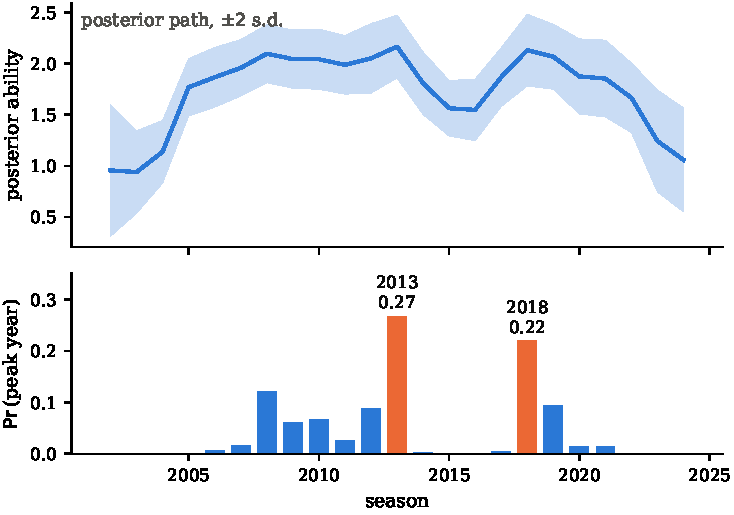
\includegraphics[width=0.86\textwidth]{nadal.pdf}
\caption{Rafael Nadal's posterior ability path from 1{,}317 matches
(top) and the law of its argmax (bottom). The path is one broad
plateau and the argmax law is bimodal, at 2013 and 2018, with the
seasons between them carrying almost no mass. The band in the top
panel does not contain that statement, and no summary of the yearly
marginals does either.}
\label{fig:nadal}
\end{figure}

Figure~\ref{fig:nadal} puts the two objects on one time axis. The
mechanism behind the second feature is visible in the same fit.
At equal posterior mean, the year with fewer matches carries more
argmax mass, because fewer matches leave a wider posterior and a
wider posterior has more room to hold the maximum. Nadal's 2010 has
posterior mean $2.042$ from 80 matches and probability $0.066$; his
2012 has mean $2.051$ from 48 matches and probability $0.088$. A
table of yearly ratings with error bars does not contain that
comparison, because the comparison is between joint events.

Two hundred thousand draws from each posterior referee the exact
pass, with maximum discrepancy $0.0019$ across all six careers and
every year. The Gaussian posterior is approximate, as it is in every
rating system that reports one. The query on that posterior is not.

\section{Software}

The factor win node, its top-$k$ relatives, both Jacobian blocks and
the calibration inverses ship in the \texttt{winning} package of
\citet{cotton2026}: a Python reference with R, JavaScript, Julia and
Rust ports pinned to embedded parity vectors, most at $10^{-15}$. The observed win node,
likelihood \eqref{eq:obslik} with analytic score, is the estimation
core of \texttt{MultinomialProbit.jl}, whose score is additionally
refereed by forward-mode automatic differentiation through the same
code path. The chain and band layer is \texttt{GMRFExtremes.jl},
which reads a Gauss--Markov chain off a tridiagonal precision and
dispatches on GMRF library types. Wider bandwidth and general
sparsity are refused with a pointer to the lifted pass and to
\citet{bolin2015} respectively.

\section{Scope}

The reduction requires structure. Factor coupling of rank $r$ costs
a $Q$-node quadrature and is exact to quadrature accuracy; precision
bandwidth $b$ costs $O(nL^{b+1})$ and is practical for $b\le 3$;
general sparse precision gets neither treatment here, and the
excursion functionals then belong to the sampling methods of
\citet{bolin2015}. The win-node concept itself is not new: TrueSkill
carries a binary one, \citet{muller2022} derived the tie-density
derivative for absolutely continuous laws, the lattice engine and its Jacobians are
\citet{cotton2026}, and the factor query is \citet{cotton2026b}.
Equation~\eqref{eq:obslik} is the multinomial probit likelihood and
is classical, and so are the maximum and first-passage passes and
the state lift \citep{hayter2006,basak2004}. New here are the exact
argmax marginals on a data-conditioned chain and the peak-career
result of Section~\ref{sec:tennis}. We leave to future work the lifted-state
argmax at $b\ge2$ and message compression past $b\approx3$.

\begin{thebibliography}{99}

\bibitem[Armitage et~al.(1969)Armitage, McPherson, and
Rowe]{armitage1969} P.~Armitage, C.~K.~McPherson, and B.~C.~Rowe.
Repeated significance tests on accumulating data. \emph{J.\ R.\
Statist.\ Soc.\ A} 132(2):235--244, 1969.

\bibitem[Basak and Ho(2004)]{basak2004} G.~K.~Basak and K.-W.~R.~Ho.
Level-crossing probabilities and first-passage times for linear
processes. \emph{Advances in Applied Probability} 36(2):643--666,
2004.

\bibitem[Bolin and Lindgren(2015)]{bolin2015} D.~Bolin and
F.~Lindgren. Excursion and contour uncertainty regions for latent
Gaussian models. \emph{J.\ R.\ Statist.\ Soc.\ B} 77(1):85--106,
2015.

\bibitem[Bolin and Lindgren(2018)]{bolin2018} D.~Bolin and
F.~Lindgren. Calculating probabilistic excursion sets and related
quantities using excursions. \emph{Journal of Statistical Software}
86(5):1--20, 2018.

\bibitem[Cotton(2026a)]{cotton2026} P.~Cotton. Scalable inversion of
contests with correlated performances, including softmax and
multinomial probit. arXiv:2609.01133, 2026. Reference implementation
and parity-locked ports: \texttt{github.com/microprediction/winning}.

\bibitem[Cotton(2026b)]{cotton2026b} P.~Cotton. Deterministic
probabilities for Thompson sampling and entropy search. Working paper,
2026.

\bibitem[Coulom(2008)]{coulom2008} R.~Coulom. Whole-history rating: a
Bayesian rating system for players of time-varying strength. In
\emph{Computers and Games}, Lecture Notes in Computer Science 5131,
pages 113--124. Springer, 2008.

\bibitem[Domencich and McFadden(1975)]{domencich1975} T.~Domencich
and D.~McFadden. \emph{Urban Travel Demand: A Behavioral Analysis}.
North-Holland, 1975.

\bibitem[Hayter(2006)]{hayter2006} A.~J.~Hayter. Recursive integration
methodologies with statistical applications. \emph{Journal of
Statistical Planning and Inference} 136(7):2284--2296, 2006.

\bibitem[Herbrich et~al.(2007)Herbrich, Minka, and
Graepel]{herbrich2007} R.~Herbrich, T.~Minka, and T.~Graepel.
TrueSkill: a Bayesian skill rating system. In \emph{Advances in
Neural Information Processing Systems~19}, pages 569--576. MIT Press,
2007.

\bibitem[Miwa et~al.(2003)Miwa, Hayter, and Kuriki]{miwa2003}
T.~Miwa, A.~J.~Hayter, and S.~Kuriki. The evaluation of general
non-centred orthant probabilities. \emph{J.\ R.\ Statist.\ Soc.\ B}
65(1):223--234, 2003.

\bibitem[Mori et~al.(2021)Mori, Majumdar, and Schehr]{mori2021}
F.~Mori, S.~N.~Majumdar, and G.~Schehr. Distribution of the time of
the maximum for stationary processes. \emph{EPL} 135(3):30003, 2021.

\bibitem[M\"uller et~al.(2022)M\"uller, Nesterov, and
Shikhman]{muller2022} D.~M\"uller, Y.~Nesterov, and V.~Shikhman.
Discrete choice prox-functions on the simplex. \emph{Mathematics of
Operations Research} 47(1):485--507, 2022. arXiv:1909.05591.

\bibitem[Ridgway(2016)]{ridgway2016} J.~Ridgway. Computation of
Gaussian orthant probabilities in high dimension. \emph{Statistics
and Computing} 26(4):899--916, 2016.

\end{thebibliography}

\end{document}
